\chapter{Write Away 4}

\begin{figure}[H]
    \centering
    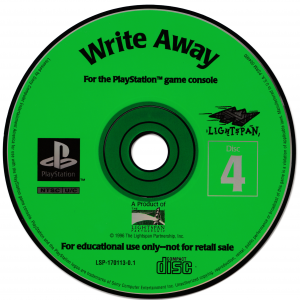
\includegraphics[width=\textwidth/2]{./Games/WriteAway/Images/WriteAway4CD.png}
    \caption{Write Away 4 CD}
\end{figure}

The fourth of the ten Write Away games published and released by The Lightspan Partnership for the PlayStation 1.

Write Away 4 features ten video programs, including an introduction video, eight story videos, and a conclusion video:

\begin{itemize}
    \item Write Away Episode Four Introduction
    \item The Fearless Lion by Desirae Hernandez
    \item The Earth by Jasmine Walker
    \item Supersurf by James Mungo
    \item Good Night to All by Stacy Winn
    \item The Test by Brad Sherwood
    \item The Storm by Mark Herman
    \item The Dancing Princess by Tara Brechun
    \item Attack of the Ninja Junkfood by Colin Devane
    \item Write Away Conclusion
\end{itemize}

\clearpage
\newpage

\section{Transcriptions}

\subsection{The Fearless Lion by Desirae Hernandez}

BRIAN:
Okay Joe, okay.
Look at this wrapping!

JOE:
Give it to me!
See?
It's a lion, the king of the jungle, my favorite animal.
I got it for you.

SCOUT, TRESSY, PAUL:
We!

JOE:
We got it for you.

BRIAN:
What's this?

JOE:
Oh, that's a story that I...
We read that made us decide to buy you that neat lion.
It tells all about teamwork and how it can solve any problem.

SCOUT, TRESSY, PAUL:
And\dots

JOE:
And how being honest with your friends can make everything turn out all right in the end.
It comes to us from second-grader Desiree Hernandez from Alameda Elementary in Las Cruces, New Mexico.
Now let's all listen to the roar of 'The Proud and Fearless Lion'.

SCOUT (VOICE OVER)
There once lived a proud and fearless lion.

LION:
Yeah.
I ain't afraid of nothing.
Not a bird nor a mouse.

SCOUT (VOICE OVER):
Now the problem was that every night at the same time, he would go into the jungle and roar.

LION:
ROAR!

SCOUT (VOICE OVER):
This made the other animals really mad because his roaring woke them up.

LION:
ROAR!

SCOUT (VOICE OVER):
So the angry animals held a meeting to decide how to stop the lion from roaring.

ELEPHANT:
I'm so tired, I can't get any sleep!

MONKEY:
Me either, and I need my beauty rest.

TIGER:
You're right.
You're both right.

ELEPHANT:
I think we should make the lion move away.

MONKEY, TIGER:
Too dangerous!

MONKEY:
I think we should scare him away.

ELEPHANT, TIGER:
Too stupid!

TIGER:
I've got it!
Why don't we just ask him to stop roaring at night?

ELEPHANT, MONKEY:
Perfect!

TIGER:
Mr. Lion
We have come to ask you to please stop roaring at night.
You're keeping all of the animals of the jungle awake.

LION:
I am?

MONKEY:
Yeah, and furthermore -

LION:
Well why didn't you just say so?
I'm sorry.
Hey, tell you what?
From now on I'll only roar in the mornings.

SCOUT (VOICE OVER):
And so from that day on, the animals got their sleep, and The Fearless Lion roared at the beginning of each day\dots

LION:
ROAR!

SCOUT (VOICE OVER):
\dots to wake the animals up.

\subsection{The Earth by Jasmine Walker}

TRESSY:
Hey Brian!
I know how much you love to travel, so I got you a globe so you can see all the places that you're going to.

BRIAN:
Thanks!

TRESSY:
Yeah.

BRIAN:
This is perfect.
Wow, is it amazing how big the Earth seems?

TRESSY:
Yeah.

BRIAN:
When you look at it like this.

TRESSY:
Mhh hmm.

BRIAN:
Hey you guys, look!
I got a globe.

TRESSY:
The Earth may seem big to you and me, there's so much to see.
The Earth is important to us because it's where we live, and that's why we need to take very good care of it.
I want to share this story with you written by first-grader Jasmine Walker from Town Point Elementary.
Let's see how Jasmine describes all the reasons she loves the Earth.

TRESSY (FROM THE STORY):
I feel good because I live on the Earth.
The Earth has gravity.
The Earth is blue and green.
The Earth has air.
The Earth has farms.
The Earth has schools.
The Earth has trees.
And best of all, the Earth has people on it.
The Earth.
The end.

\subsection{Supersurf by James Mungo}

JOE:
That was great!

PAUL:
Hi everybody!

JOE, BRIAN, SCOUT, TRESSY:
Hey! Hi!

PAUL:
Hey, I thought this was a party?
I know I'm late, but come on, let's party hardy!

JOE, SCOUT, TRESSY:
Yeah!

BRIAN:
Hey you guys, where you going?

PAUL:
Hey Brian, I brought you a present.

BRIAN:
Do I know you?

PAUL:
Yes, remember?
I'm the brave individual that saved you when you went skateboarding out of control at a wind velocity much too fast for your body type.

BRIAN:
I do remember you now.
You saved my life!
Thanks Guy!

PAUL:
No problemo.
Hey look, I brought you this gift.
This will help you express your wild side, but be on a safer [ride] too.

BRIAN:
Wow, thanks a lot!
Look everyone, a boogie board!
Cowabunga!

PAUL:
I bet he never expected to get such a rad gift from someone like me.
When you create interesting characters like myself, you can put them in all kinds of unlikely situations, and that makes your story so much more fun.
That's exactly what our next author did - created a unique character that becomes a very unlikely hero.
It comes from fifth-grader James R. Mungo of Linda Vista Elementary School in Mission Viejo.
Let's meet the one, the only, Supersurf!

TRESSY (VOICE OVER):
Once upon a time, there was a surfer named Supersurf.
No one knew his real name.
Over the summer and spring, he surfed.
During fall and winter, he drove an ice cream truck.
One day, after surfing, he was at home eating when suddenly his surf alarm went off.

SURF ALARM:
Big trouble at the beach!

SUPERSURF:
Oh no, trouble at the beach!
I must go!

TRESSY (VOICE OVER):
When he got to the beach, he saw what the trouble was.

SUPERSURF:
Oh, it's a giant shark scaring people!
Everyone get out of the water, 'cause I'm going in!

TRESSY (VOICE OVER):
He jumped into the water and wrestled the shark until it swam away.

SANDY:
Oh, you saved my life!

EUNICE:
Mine too!

SANDY:
Whatever!
My name is Sandy, what's yours?

SUPERSURF
Supersurf.

SANDY:
No, I mean your real name.

SUPERSURF:
Supersurf, okay.
Gotta go home to eat now.

EUNICE:
He's so big and strong, and he was looking at me!

SANDY:
No way, he was looking at me!

EUNICE:
He was looking at me!

SANDY:
He was looking at me!

EUNICE:
Me, me, me!
Buy me a snow cone?

SANDY:
Ugh, whatever.

TRESSY (VOICE OVER):
Supersurf was eating pizza and watching TV.

SUPERSURF:
I'd like to buy a vowel, Pat.
Ha ha, cool!

TRESSY (VOICE OVER):
Suddenly, the doorbell rang. Supersurf answered it.

SUPERSURF:
Yeah?

DOOR TO DOOR SALESMAN:
Would you be interested in buying a vacuum?

SUPERSURF:
No.

DOOR TO DOOR SALESMAN:
Would you be interested in buying a vacuum?

SUPERSURF:
Weren't you just here, dude?

DOOR TO DOOR SALESMAN:
No I wasn't.

SUPERSURF:
Okay cool.

TRESSY (VOICE OVER):
Suddenly, the surf alarm went off again.

SURF ALARM:
Big trouble at the beach. *inaudible*

SUPERSURF:
Oh no, not again!

TRESSY (VOICE OVER):
Back at the beach, Supersurf saw it - a beached whale!
Sandy and Eunice tried to roll the whale back into the water, but they couldn't.

SUPERSURF:
Everyone back, I'll handle this.

SANDY:
Oh, Supersurf, you saved the whale!
Oh, you're so strong!

SUPERSURF:
Whatever, I'm hungry, time for dinner.
Bye girls.

TRESSY (VOICE OVER):
And so Supersurf ate his dinner, read a book called "The Sailor Dog", and went to bed.

SUPERSURF:
[Baa waa] little doggy dude, ha ha ha.
Just another day for Supersurf!

\subsection{Good Night to All by Stacy Winn}

PAUL:
Hi, come on one word.

SCOUT, TRESSY, PAUL, BRIAN:
Two syllables\dots

PAUL:
Yeah!

SCOUT, TRESSY, PAUL, BRIAN:
Sounds like\dots
Uh\dots
Drink?
Pour? Pour! Pour! Pour!

BRIAN:
Store? Uh, gore?
For?
Uh, door?

SCOUT:
Poem!

TRESSY, PAUL, BRIAN:
Yes!

SCOUT:
That's amazing, because that's exactly what I got you for your birthday.
I wrote you a poem.

BRIAN:
Oh, okay.

SCOUT:
And here's how it goes:

Brian, oh Brian, I'ma writin' and I'ma tryin',
To let you know I'm not lying when I say you're cool, oh Brian.
The end.

BRIAN:
Yeah

SCOUT:
Thanks.
You know, it is tough to write the perfect poem to express how you feel.
You have to have exactly the right words to let people know what you mean.
I got the inspiration from my poem from an author who sent a wonderful one to us, from Stacy Winn from Lakeview School.
So listen to her wonderful poem, as we hear 'Good Night to All'.
Paul, I'm going to get you.

SCOUT (AS POET)
Good night to The Shining Moon.
Good night to the little raccoon.
Good night to the squirrel in the trees.

RACCOON:
Good night.

SCOUT (AS POET):
Good night to the ants and the bees.

ANT:
Bzzz.

SCOUT (AS POET):
Good night to the meadows breeze.
Good night to the deep blue seas.
Good night to the dog in his house.
Good night to the world as quiet as a mouse.
Good night to all.
The end.

\subsection{The Test by Brad Sherwood}

JOE:
Hey Brian!

BRIAN:
Hi!

JOE:
I'm sorry, but I don't have a present for you.
I had to make my science experiment perfect, and it took too much time.

BRIAN:
That's okay, the present doesn't matter.
You're here, and that's what counts.
And besides, getting good grades is important.

SCOUT (OFF SCREEN):
Ow, you\dots

BRIAN:
Uh oh!

JOE:
Well it sure is important.
You know, sometimes it's hard for us to decide what we should do - play or study, eat or study, watch TV or study.
The choices never end, but there's always time to play.
I like to do my work first - that way, there's always plenty of time to do all sorts of fun things.
I was reminded of this when I read the story by fourth-grader Brad Sherwood from Villa Park Elementary.
We can all learn a lesson from 'That Test'.

BRIAN (VOICE OVER):
Once there was a boy named Dan.
Now, Dan liked to skip homework and play baseball instead.

MOM:
Dan, is your homework done?

DAN:
Uh, yes Mom.

BRIAN (VOICE OVER):
Dan loved baseball.
He loved to watch it, but he would never get his homework done.

DAN:
Oh, the game's on TV.
I'll do this homework later.

BRIAN (VOICE OVER):
At school, Dan found out there was going to be a test.

TEACHER:
Okay students, listen up.
Today we're going to have a test on everything we've learned this week.
Now, the one who gets the highest score will win two tickets to the Giants game -

DAN, CHILD 1, PAULA:
Oh wow!

TEACHER:
- and\dots the chance to get their autograph.

DAN, CHILD 1, PAULA:
Oh yes!

DAN:
The Giants?
I gotta win those tickets!

CHILD 1:
I think I'm gonna win.
I've been doing all my homework and studying really hard.

PAULA:
Dan, you can't win.
You never study.
Whenever we ask you to go to study hall with us, you always say no, I'd rather play baseball.

DAN:
You're right, I should have studied harder.

TEACHER:
Okay students now: here here here.
Let's begin.

BRIAN (VOICE OVER):
The next day, the students found out the test results.

TEACHER:
Okay students, we have a winner.
It's\dots Paula, with a perfect 100.

PAUL:
Oh, thank you so much.

TEACHER:
Congratulations, Paula!
Oh, it's Time For Recess!

BRIAN:
Congratulations Paula.
Have fun at the game.

CHILD 1:
Yeah, guess what?
My dad and I are going to the game too.

PAULA:
Oh, you know what, Dan?
My dad can't go with me to the game because he's gonna be out of town that week, so you want to go with me?

BRIAN:
Would I?
Sure

PAULA:
Okay, but only if you promise to go to study group with us and to try a lot harder.

BRIAN:
I promise

PAULA:
Okay.

BRIAN (VOICE OVER):
Dan learned his lesson.
He would never forgot to do his homework again, and he would always do his best.

\subsection{The Storm by Mark Herman}

SCOUT, TRESSY, PAUL, PAUL:
Happy birthday, Brian!

BRIAN:
Thank you.

SCOUT:
Blow out the candles!

BRIAN:
Hey, how many candles did you put on this cake?
I'm not that old.

TRESSY:
I know, but it's better to have too many candles than none at all.
Have you ever been caught without candles, like, let's say, during a blackout, and you can't see at all?
I have, and I remember the important thing is to stay calm and be prepared in an emergency.
Third-grader Mark Herman from Henry Elementary reminds us to stay calm in his thrilling story, "The Storm."

JOE (VOICE OVER):
It was a Friday.
A nice day, until there were lots of clouds and heavy rainfall.
The winds were strong.

MARK:
The weather's not good Mom.
Look, the winds blew off the Smith's garage door!

MOM:
Well, when are you coming home, dear?

DAD:
I, I don't know.
The building next door got struck by lightning.
Just got hit again.
Everybody has to stay inside.
You and Mark aren't scared, are you?

MON:
Oh, no dear - oh no!
The lights just went out.

DAD:
Look, I want you to wait out at grandma's and wait out the storm.
I'll get there as soon as I can.
Goodbye, honey.

MOM:
Goodbye, dear.
We'll go to Grandma's house.

MARK:
Okay.

MOM:
It'll be fun.

MARK (NARRATING):
So we went to Grandma's house and ate dinner.

GRANDMA:
You call this a storm?
Well I remember the storm of 1890.
We all had to walk 10 miles to school barefoot, tied together by a rope, with no coats and no umbrellas.
Yeah, there we were, dodging cows and pigs and uprooted trees, and they were so cold that my ears, I couldn't even feel them anymore.
But I was never afraid because I was prepared.
I always carried my water, my flashlight, my trusty candles, and above all, my powdered eggs.
Eat up!

* knock on door *

GRANDMA:
Come in.
Oh, there he is, the hunky Power Man!

POWER MAN:
Hi everyone.
As you can see, the lights are back on, and it's safe to go outside.
Are those powdered eggs?

MARK (VOICE OVER):
Yeah, finally, my dad arrived!

MARK:
Oh Dad, you made it!

DAD:
Oh, were you scared?

MARK:
Oh, a little.

MOM:
Oh, we can go home now.

MARK:
Yeah, thanks, grandma, and I'll always remember to have plenty of flashlights and candles.

GRANDMA:
And don't forget the powdered eggs.

DAD:
Powdered eggs?

MARK (VOICE OVER):
Foreign cable TV came back on, and we were back to normal again, but none of us would ever forget the storm.
The end.

\subsection{The Dancing Princess by Tara Brechun}

BRIAN:
I'd love to dance because it's a good way to express how you feel
Just look.
You know, they're dancing reminds me of a very creative story where the main character just can't stop dancing.
It comes to us from second grader Tara Brechun of Rios Elementary in San Diego, California.
Let's watch the dancing princess.

PAUL (VOICE OVER):
Once upon a time, there lived a king, a queen, and a princess.
The king and queen enjoyed a quiet life, but their daughter always danced.
She danced when she was happy.
She danced when she was sad.
She danced all the time, and this drove the king and queen crazy.

KING:
Daughter, you must stop dancing.
You'll pass out.

QUEEN:
You'll get too thin.

KING:
Look at your mother and I.
We can dance.
And we can stop.
You see?
Dance. Stop. Dance. Stop.
So stop.

PRINCESS:
Oh Father, I can't stop dancing.
I love it so.

PAUL:
Well this went on for a very long time until one day there came a knock at the door and in stepped the prince.
The prince said\dots

PRINCE:
Stop dancing.

PAUL (VOICE OVER):
The princess took one look at the prince and stopped dancing.

PRINCE:
You must be the dancing princess.
Will you marry me?

PRINCESS:
I will, and I promise to only dance again at our wedding.

PAUL (VOICE OVER):
Now the king and queen were very happy.

QUEEN:
Where did you find him?

KING:
In the Yellow Pages.

QUEEN:
Ah, you're so clever.

PAUL (VOICE OVER):
And they all danced -

KING, QUEEN, PRINCESS, PRINCE:
Uh uh uh!

PAUL (VOICE OVER):
They all lived happily ever after.
The end.

\subsection{Attack of the Ninja Junkfood by Colin Devane}

SCOUT:
Oh! Goodness, oh!
Too much sugar!
I told them not to eat so much sugar, but would they listen to me?
No, I'm just the caterer.
I could try some carrot sticks, but no, and now look at the party.
Moderation is the key when you eat candy, you could eat a little bit, but in moderation.
I learned this important lesson from a Fifth Grader by the name of Colin Devane from Roch Courages Elementary Schools in Fountain Valley, California.
Come with us, as we learn about moderation as we see the attack of the Ninja Junkfood.
Hayah!

PAUL (VOICE OVER):
One day in the castle of Lord Ice Cream Sunday, his majesty shouted.

LORD ICE CREAM SUNDAY:
I must take over Lord [Norfolk]'s Kingdom, steal his transmogrifier box, then I will turn his tofu man into a candy bar.
And then I will turn Lord Low Fat Milk into a stick of butter.
Ha ha ha ha ha.

BEEF CHUCKIE BOB:
But your majesty -

LORD ICE CREAM SUNDAY:
What is it is my trusted psychic, Beef Chuckie Bob.

BEEF CHUCKIE BOB:
Lord Low-Fat Milk's Army is very powerful, and could easily overpower us with his tofu man.

LORD ICE CREAM SUNDAY:
I know that, you nut case.
That's why I rounded up Neapolitan Ninja to fight for us.

BEEF CHUCKIE BOB:
But your majesty, what if Lord Low-Fat Milk's spy, Baked Unsalted Sunflower Seed, should overhear us and ruin all our plans.

LORD ICE CREAM SUNDAY:
That's why I added butter to the bacon, double the glaze on the donuts, deep-fried the potato chips, and tripled the security.
I also changed the password.

BEEF CHUCKIE BOB:
You mean the password cholesterol.

LORD ICE CREAM SUNDAY:
Shh!
Now, to prepare.

BEEF CHUCKIE BOB:
Yeah.

PAUL (VOICE OVER):
Sunflower Seed's spy had been listening to it all.

BAKED UNSALTED SUNFLOWER SEED:
I better skedaddle back to Lord Low-Fat Milk, and tell them all I've heard.
Sir, pant, pant, pant.
I've been spying on Lord Ice Cream Sundae.
He's planning on attacking the castle at dawn.
He's gonna try to steal the Royal transmogrifier box and turn us all into candy bars and you butter.
And he's using Neapolitan Ninja.

LORD LOW-FAT MILK:
Have no fear, our arteries are clear.
We'll be ready because I have a plan.
Hello, testing, hello.
Everyone in my kingdom!
Quick into your fridge, turn up the heaters, and melt any ice cream that comes our way.
Now, Sunflower Seeds Spy, go get our secret weapon.
Tofu man.

LORD ICE CREAM SUNDAY:
Alright, we're outside Lord Low-Fat Milk's Castle.
Ooh, you can smell the skimmed milk.
Makes me want to curdle.
All right, you big, stinky, gooey cavity-causing ninja, attack!

LORD LOW-FAT MILK:
All right, tofu man
You must save the right of every person to have proper nutritious food where they want to.
Don't do it for me, we'll do it for all the millions of toothless children out there who want to have healthy teeth and gums, not to mention nice waistlines.
Go! Save Our Kingdom!

TOFU MAN:
Never fear, tofu is here!
Neapolitan ninja, do you give up?

NEAPOLITAN NINJA:
Never, take this!

TOFU MAN:
Uh, that was disgusting.
Here, have these carrot sticks.

NEAPOLITAN NINJA:
Ugh, peuch!
It burns! It burns!
Take this whipped cream.

TOFU MAN:
It's not even fat-free!
How low will you go?

NEAPOLITAN NINJA:
And now to finish you up with a maraschino cherry.
What's that I feel?
You have turned the heater on!
I'm melting!
I'm melting!
What a world!
What a world!

TOFU MAN:
Ha ha ha ha ha.

BEEF CHUCKIE BOB:
We lost, your majesty.
The Neapolitan ninja is no more.
Where will we go?
What will we do?

LORD ICE CREAM SUNDAY:
Well, you would probably be a doggie treat for some [mingie muk] now, but I\dots
I\dots
\dots I changed my ways.
You can't make everyone like you, so I've decided to divide my kingdom up into three sections: regular, low-fat, and fat-free ice creams.
And then they'll like me.
They'll really like me.

BAKED UNSALTED SUNFLOWER SEED:
Sire, we've won!
Neapolitan ninja is no more, and Lord Ice Cream Sunday has surrendered!

LORD LOW-FAT MILK:
Yes, there he goes.
How can I ever thank you enough, Tofu Man?

TOFU MAN:
Glad to be of help, your highness.
All it takes is a little fruit and a side of vegetables to make them see the errors of their ways.
Carrot stick?

LORD LOW-FAT MILK:
Uh, thank you.

PAUL (VOICE OVER):
And so the kingdom was saved, wholesome food had triumphed over junk food once again.
The end.

\subsection{Write Away Conclusion}

BRIAN:
Thanks everyone for a wonderful birthday party and for all my great presents.
And thanks to all of you for the stories you submitted.

SCOUT:
And your stories are like presents to us because with each one we read, we learn something new about you, and about ourselves.

PAUL:
Through writing, we can reach across the miles to let others know how we live, and feel, and just how different and similar we are.

JOE:
So keep sending us those wonderful stories so we can share them with everyone.

TRESSY:
Come on, everybody, let's take a group shot so we'll always remember this day.

BRIAN, SCOUT, TRESSY, PAUL:
Yeah!

VOICE OVER:
All right, everyone, smile

EVERYONE:
Write away!

\section{Credits}

Executive Producers: Gregg Baker, Deborah Brucher Wren, Michael Wren;
Directors: Gregg Baker, Robin LeValley;
Technical Director: Joseph S. Abreu;
Cast: Paul David, Scout Jackson, Joe Lopez, Jr., Tressy Elise, Brian Kwan;
Writers: Deborah Brucher Wren, Robin LeValley;
Music: Rick Illes, Michael Wren;
Lighting Director: Steve Raines;
Cameras: Steve Raines, Andy Hall, Richard Crow;
Audio: Rad Corn;
Childrens Art: Blythe Baker;
Production Assistant: Sam Kephart;
Editor: Joseph S. Abreu;
Engineer: Michael Curran;
Production Coordinator: Judy Block;
Graphic Artist: Alan Scott;
Theme Song: Michael Wren;

\section{Screenshots}

\begin{figure}[H]
    \centering
    \begin{subfigure}{0.45\textwidth}
        \centering
        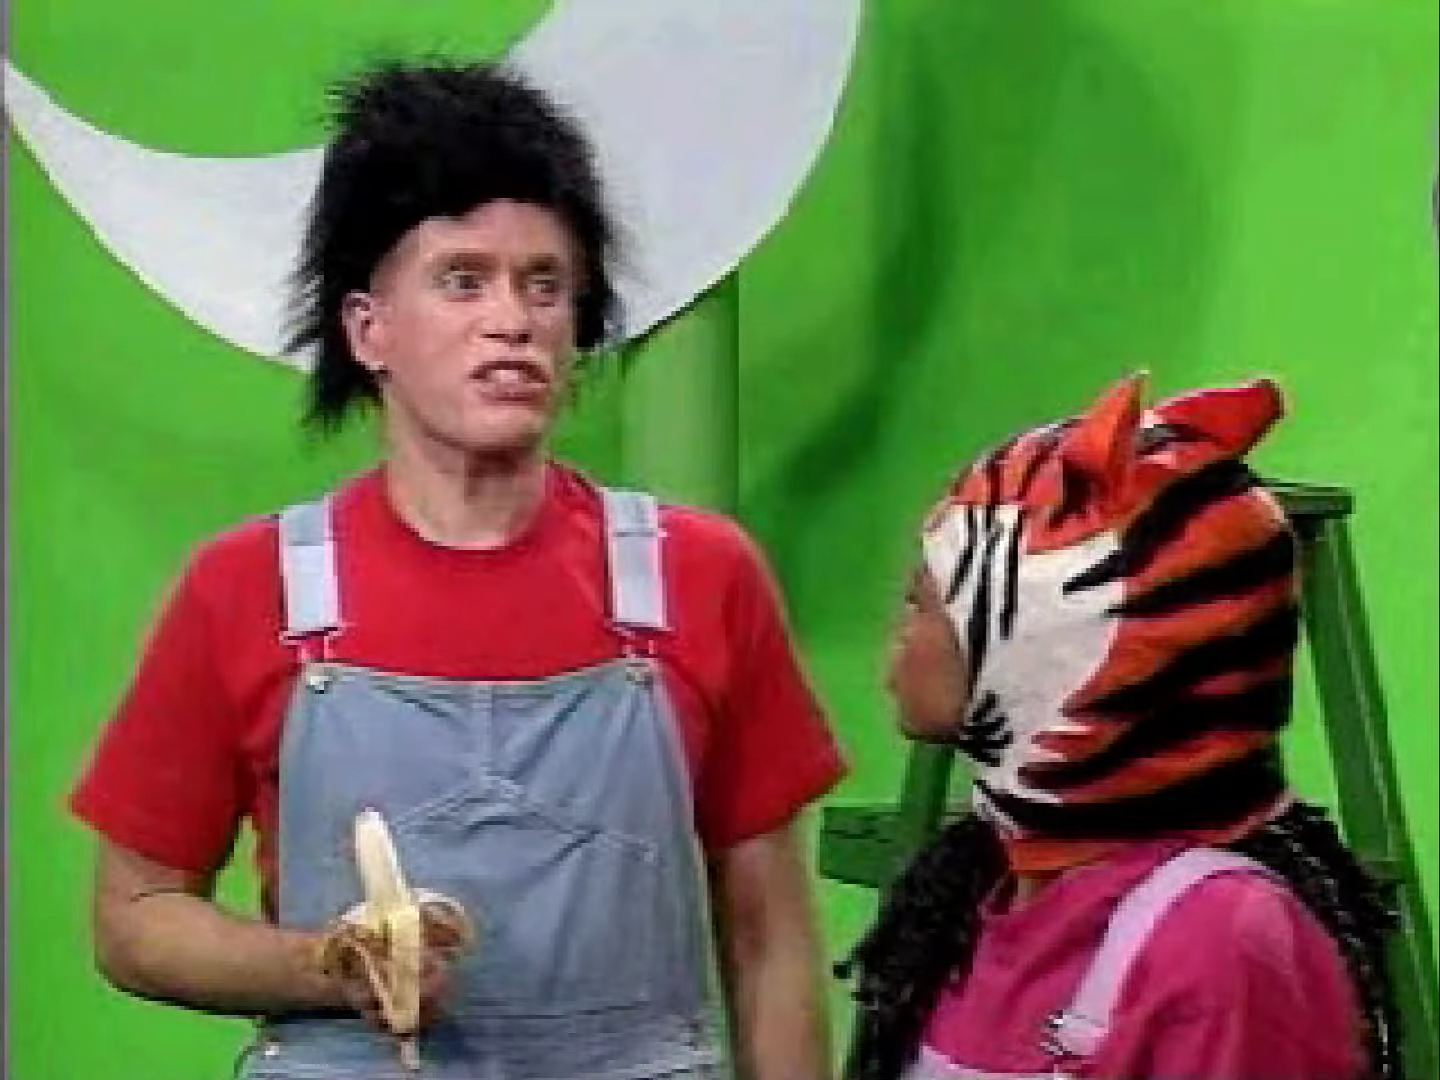
\includegraphics[width=\linewidth]{Games/WriteAway/Images/WriteAway4Screenshot1.png}
        \caption{Write Away 4 - Screenshot 1}
    \end{subfigure}
    \begin{subfigure}{0.45\textwidth}
        \centering
        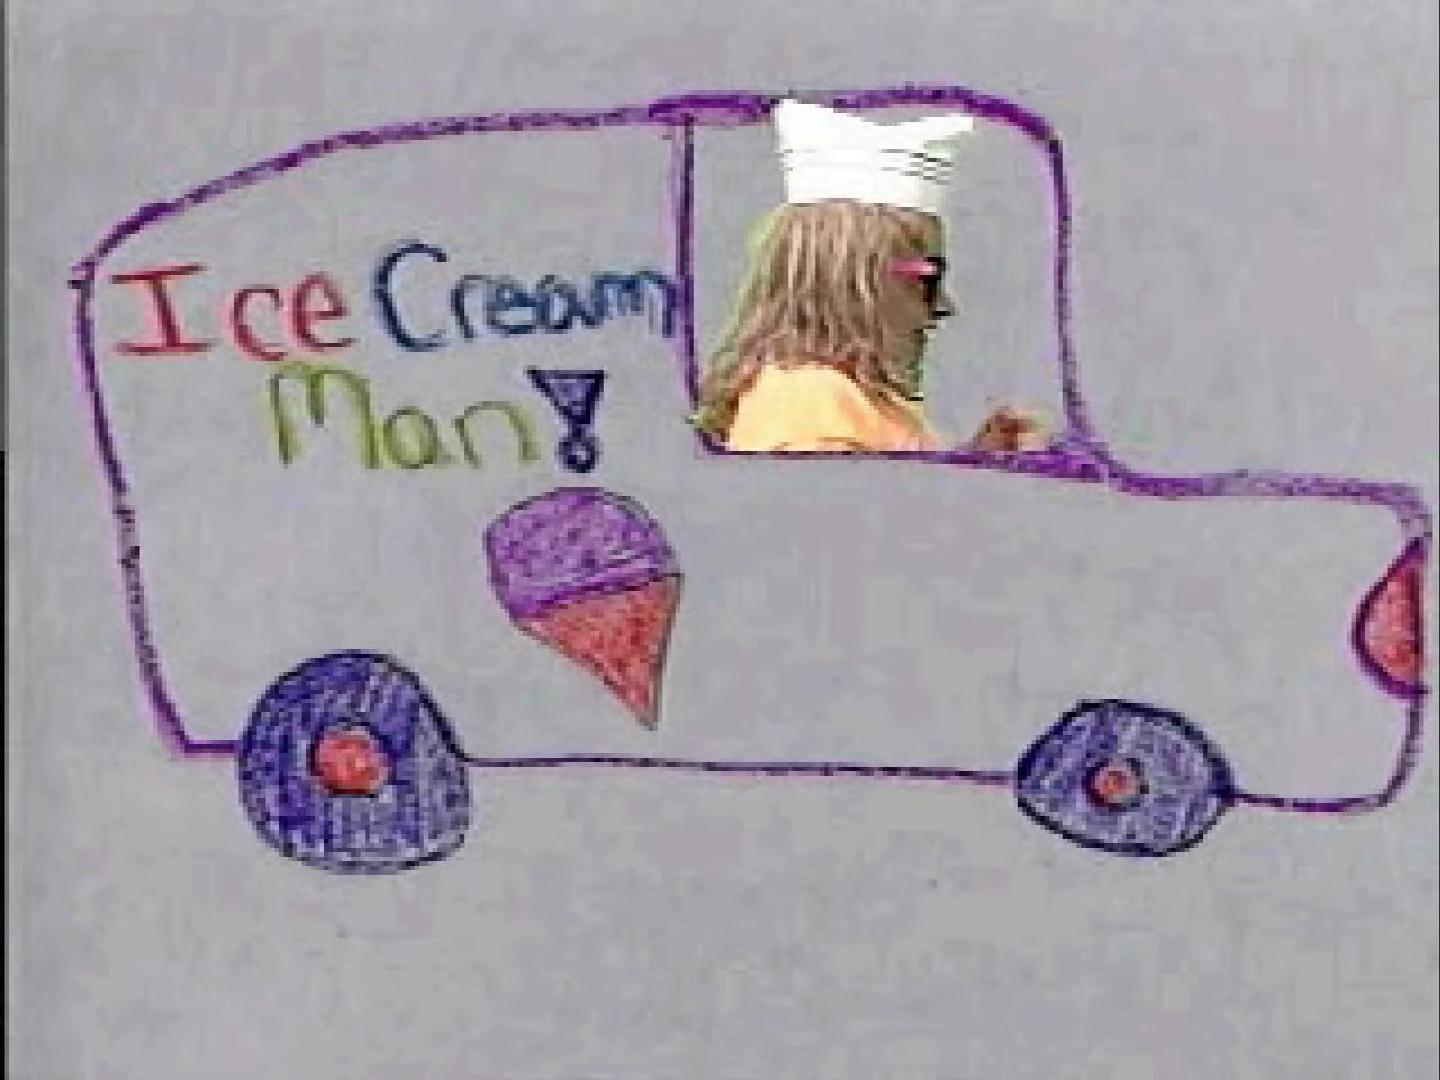
\includegraphics[width=\linewidth]{Games/WriteAway/Images/WriteAway4Screenshot2.png}
        \caption{Write Away 4 - Screenshot 2}
    \end{subfigure}

    \begin{subfigure}{0.45\textwidth}
        \centering
        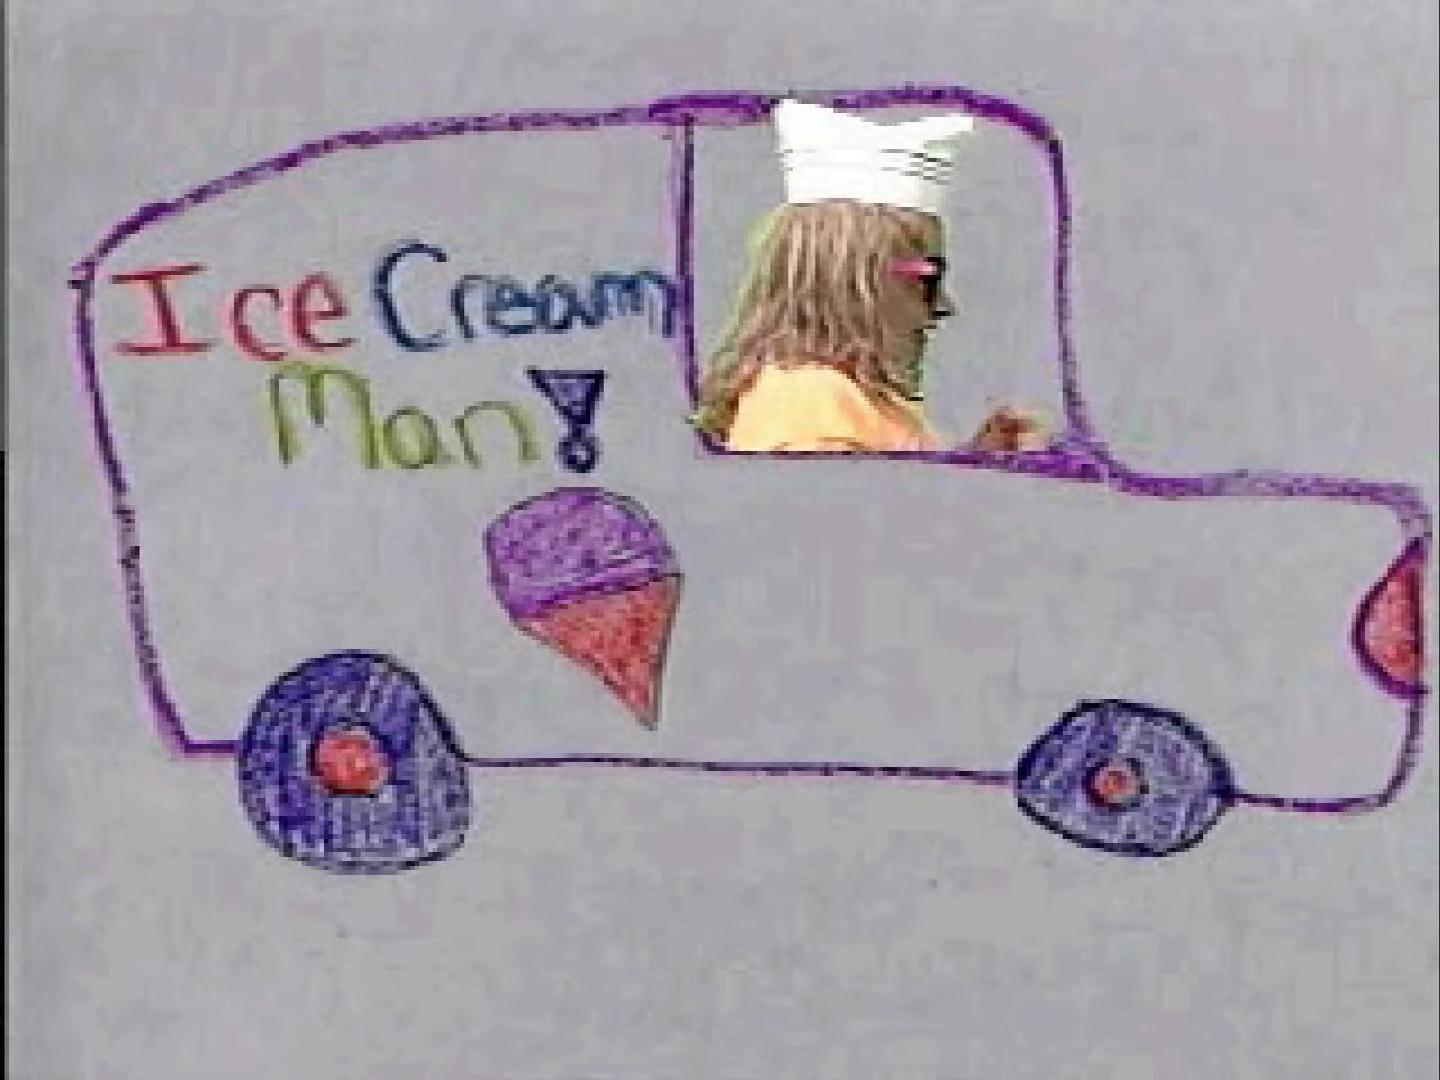
\includegraphics[width=\linewidth]{Games/WriteAway/Images/WriteAway4Screenshot2.png}
        \caption{Write Away 4 - Screenshot 3}
    \end{subfigure}
    \begin{subfigure}{0.45\textwidth}
        \centering
        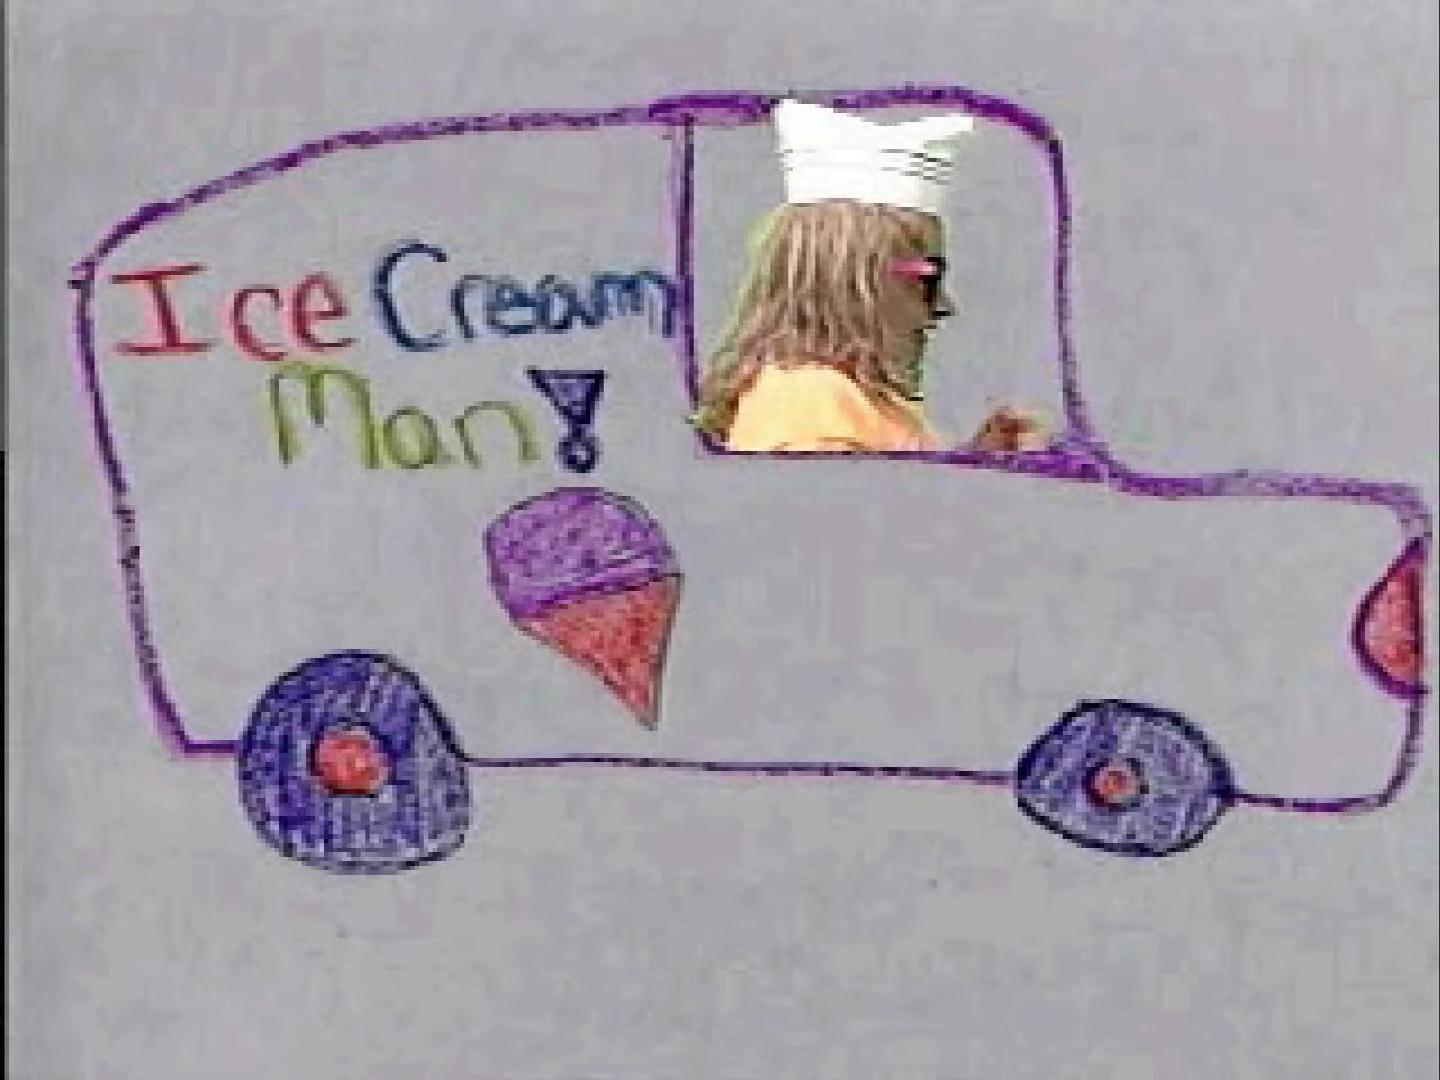
\includegraphics[width=\linewidth]{Games/WriteAway/Images/WriteAway4Screenshot2.png}
        \caption{Write Away 4 - Screenshot 4}
    \end{subfigure}
    \caption{Screenshots from Write Away 4}
\end{figure}
